\documentclass[10pt,twocolumn]{article}

\usepackage[a4paper,margin=1.5cm]{geometry}
\usepackage{authblk}
\usepackage{setspace}
\usepackage[compact]{titlesec}
\pdfoptionpdfminorversion=4
\usepackage{graphicx}
\usepackage[separate-uncertainty=true]{siunitx}
\usepackage{hyperref}
\usepackage{amsbsy,amssymb,amsmath,bm}
\usepackage[none]{hyphenat}
\usepackage{float}
\usepackage{booktabs}
\usepackage{xcolor}
\usepackage{soul}
\parskip 0.35\baselineskip
\parindent 0mm
\setlength{\textfloatsep}{0.45\baselineskip}
\setlength{\floatsep}{0.35\baselineskip}
\setlength{\intextsep}{0.35\baselineskip}
\renewcommand\refname{\vspace{-\baselineskip}}
\graphicspath{{figures/}{docs/figures/}{figures/Detector_performance_analysis_Rn222_repetition_comparison/}{docs/figures/Detector_performance_analysis_Rn222_repetition_comparison/}{figures/Detector_performance_analysis_Rn222_activity_normalized/}{docs/figures/Detector_performance_analysis_Rn222_activity_normalized/}{figures/Simulation_output_signal_inference_metrics/}{docs/figures/Simulation_output_signal_inference_metrics/}{figures/Signal_inference_metrics/}{docs/figures/Signal_inference_metrics/}}

\makeatletter
\renewcommand{\maketitle}{
\twocolumn[
  \begin{center}
    {\LARGE \@title \par}
    \vspace{0.5em}
    {\normalsize \@author \par}
    \vspace{1em}
  \end{center}
]
}
\makeatother

\title{Gamma detection for source localisation in targeted alpha therapy}

\author{
C. De Sio$^{\text{a}}$,
L. Abu Sabah$^{\text{a}}$,
J. Duan$^{\text{a}}$,
Y. Shi$^{\text{a}}$,
S. Williams$^{\text{a}}$,
J. Velthuis$^{\text{a}}$\\
\vspace{0.3em}
\small $^{\text{a}}$School of Physics, University of Bristol, Bristol, United Kingdom
}

\date{}

\begin{document}

\maketitle

\textbf{
Targeted alpha therapies can deliver high localised dose, but treatment
planning and delivery depend on whether the radionuclide source remains near
the intended site after administration.  In the
\href{https://doi.org/10.3390/biomedinformatics5040058}{AlphaGlue delivery concept}
\cite{AlphaGlue2025}, \(\alpha\)-emitters are applied to a tumour region in a
thin glue layer.  Here we present a Geant4 simulation study showing that
decay-chain gamma detection can distinguish retained, broadly diffused, and
locally displaced source states in an AlphaGlue-like geometry.  Using 50
independent repetitions, baseline-subtracted gamma-hit profiles
reconstructed the broad diffusion fraction with \(R^2=0.9987\) and about one
percentage-point mean absolute error, while localised-source residuals
identified displaced activity with mean position errors of
\(16\)--\(\SI{30}{mm}\).  These results support gamma detection as a
candidate route for emitter-position monitoring, treatment planning, and
delivery verification.
}

\subsection*{Introduction}

In targeted alpha therapy, the delivered dose is strongly local.  A treatment
plan therefore depends not only on the initial activity distribution, but also
on whether source material and progeny remain near the intended deposition
site, diffuse into surrounding tissue, or are redistributed by biological
transport~\cite{laura,heger}.  The
\href{https://doi.org/10.3390/biomedinformatics5040058}{AlphaGlue concept}
proposes suspending alpha emitters in a thin glue layer applied to tissue
\cite{AlphaGlue2025}.  The concept has previously been evaluated with
Geant4 and Geant4-DNA simulations for dose and DNA-damage modelling
\cite{Geant4,Geant4DNA}.  This study investigates whether the accompanying
gamma signal can be used as a theranostic observable, to monitor the emitter
position, detect source movement, and provide useful information as a
function of detection time.

\subsection*{Simulation model}

Photon transport was simulated with the Geant4 toolkit \cite{Geant4}.  The
model places a \(\SI{40}{mm} \times \SI{2}{mm} \times \SI{40}{mm}\)
loaded glue layer on the \(+y\) surface of a
\(\SI{20}{cm} \times \SI{20}{cm} \times \SI{150}{cm}\) water phantom.
Six detector panels surround the phantom at \(\SI{20}{cm}\) from
the water surface.  Each photon entry into a detector panel is counted as
one hit.

Seven source configurations were studied to separate three clinically relevant
possibilities: emitter retained in the loaded glue layer, emitter broadly mixed
into the surrounding volume, and emitter transported to a localised displaced
region.  The retained-source case is used as the baseline.  
As discussed in \cite{laura,heger}, some of the \(\alpha\)-emitters in the decay chain can be taken up by the blood.
\cite{laura,heger} report large variations in this uptake across different experiments, further 
emphasizing the need for local dose verification.
This is taken into account in the simulation by studying cases where
%The broad-mixing cases place 
10\%, 50\%, or 90\% of the radioisotope is placed diffusely in the water volume, while
the localised-displacement cases place 20\%, 40\%, or 60\% of the source
in a small displaced water region.  These configurations are intended as
sensitivity tests for source movement and source localisation.
%rather than a specific patient geometry.

Each configuration was simulated with 50 independent repetitions of 10,000
primary decays, giving 500,000 simulated decays per configuration and
3.5 million simulated decays across all source states.  The repeated runs
define the run-to-run uncertainty used in the residual and detectability
analysis.  Where activity-scaled observables are quoted, the simulated
decays are rescaled to a DaRT-like reference activity of
\(3~\mu\mathrm{Ci}\) (\(\SI{111}{\kilo\becquerel}\)), matching the order of a
single DaRT seed~\cite{dart}.
The simulated geometry is shown in Fig.~\ref{fig:abs_geometry}.

\begin{figure}[!tbp]
    \centering
    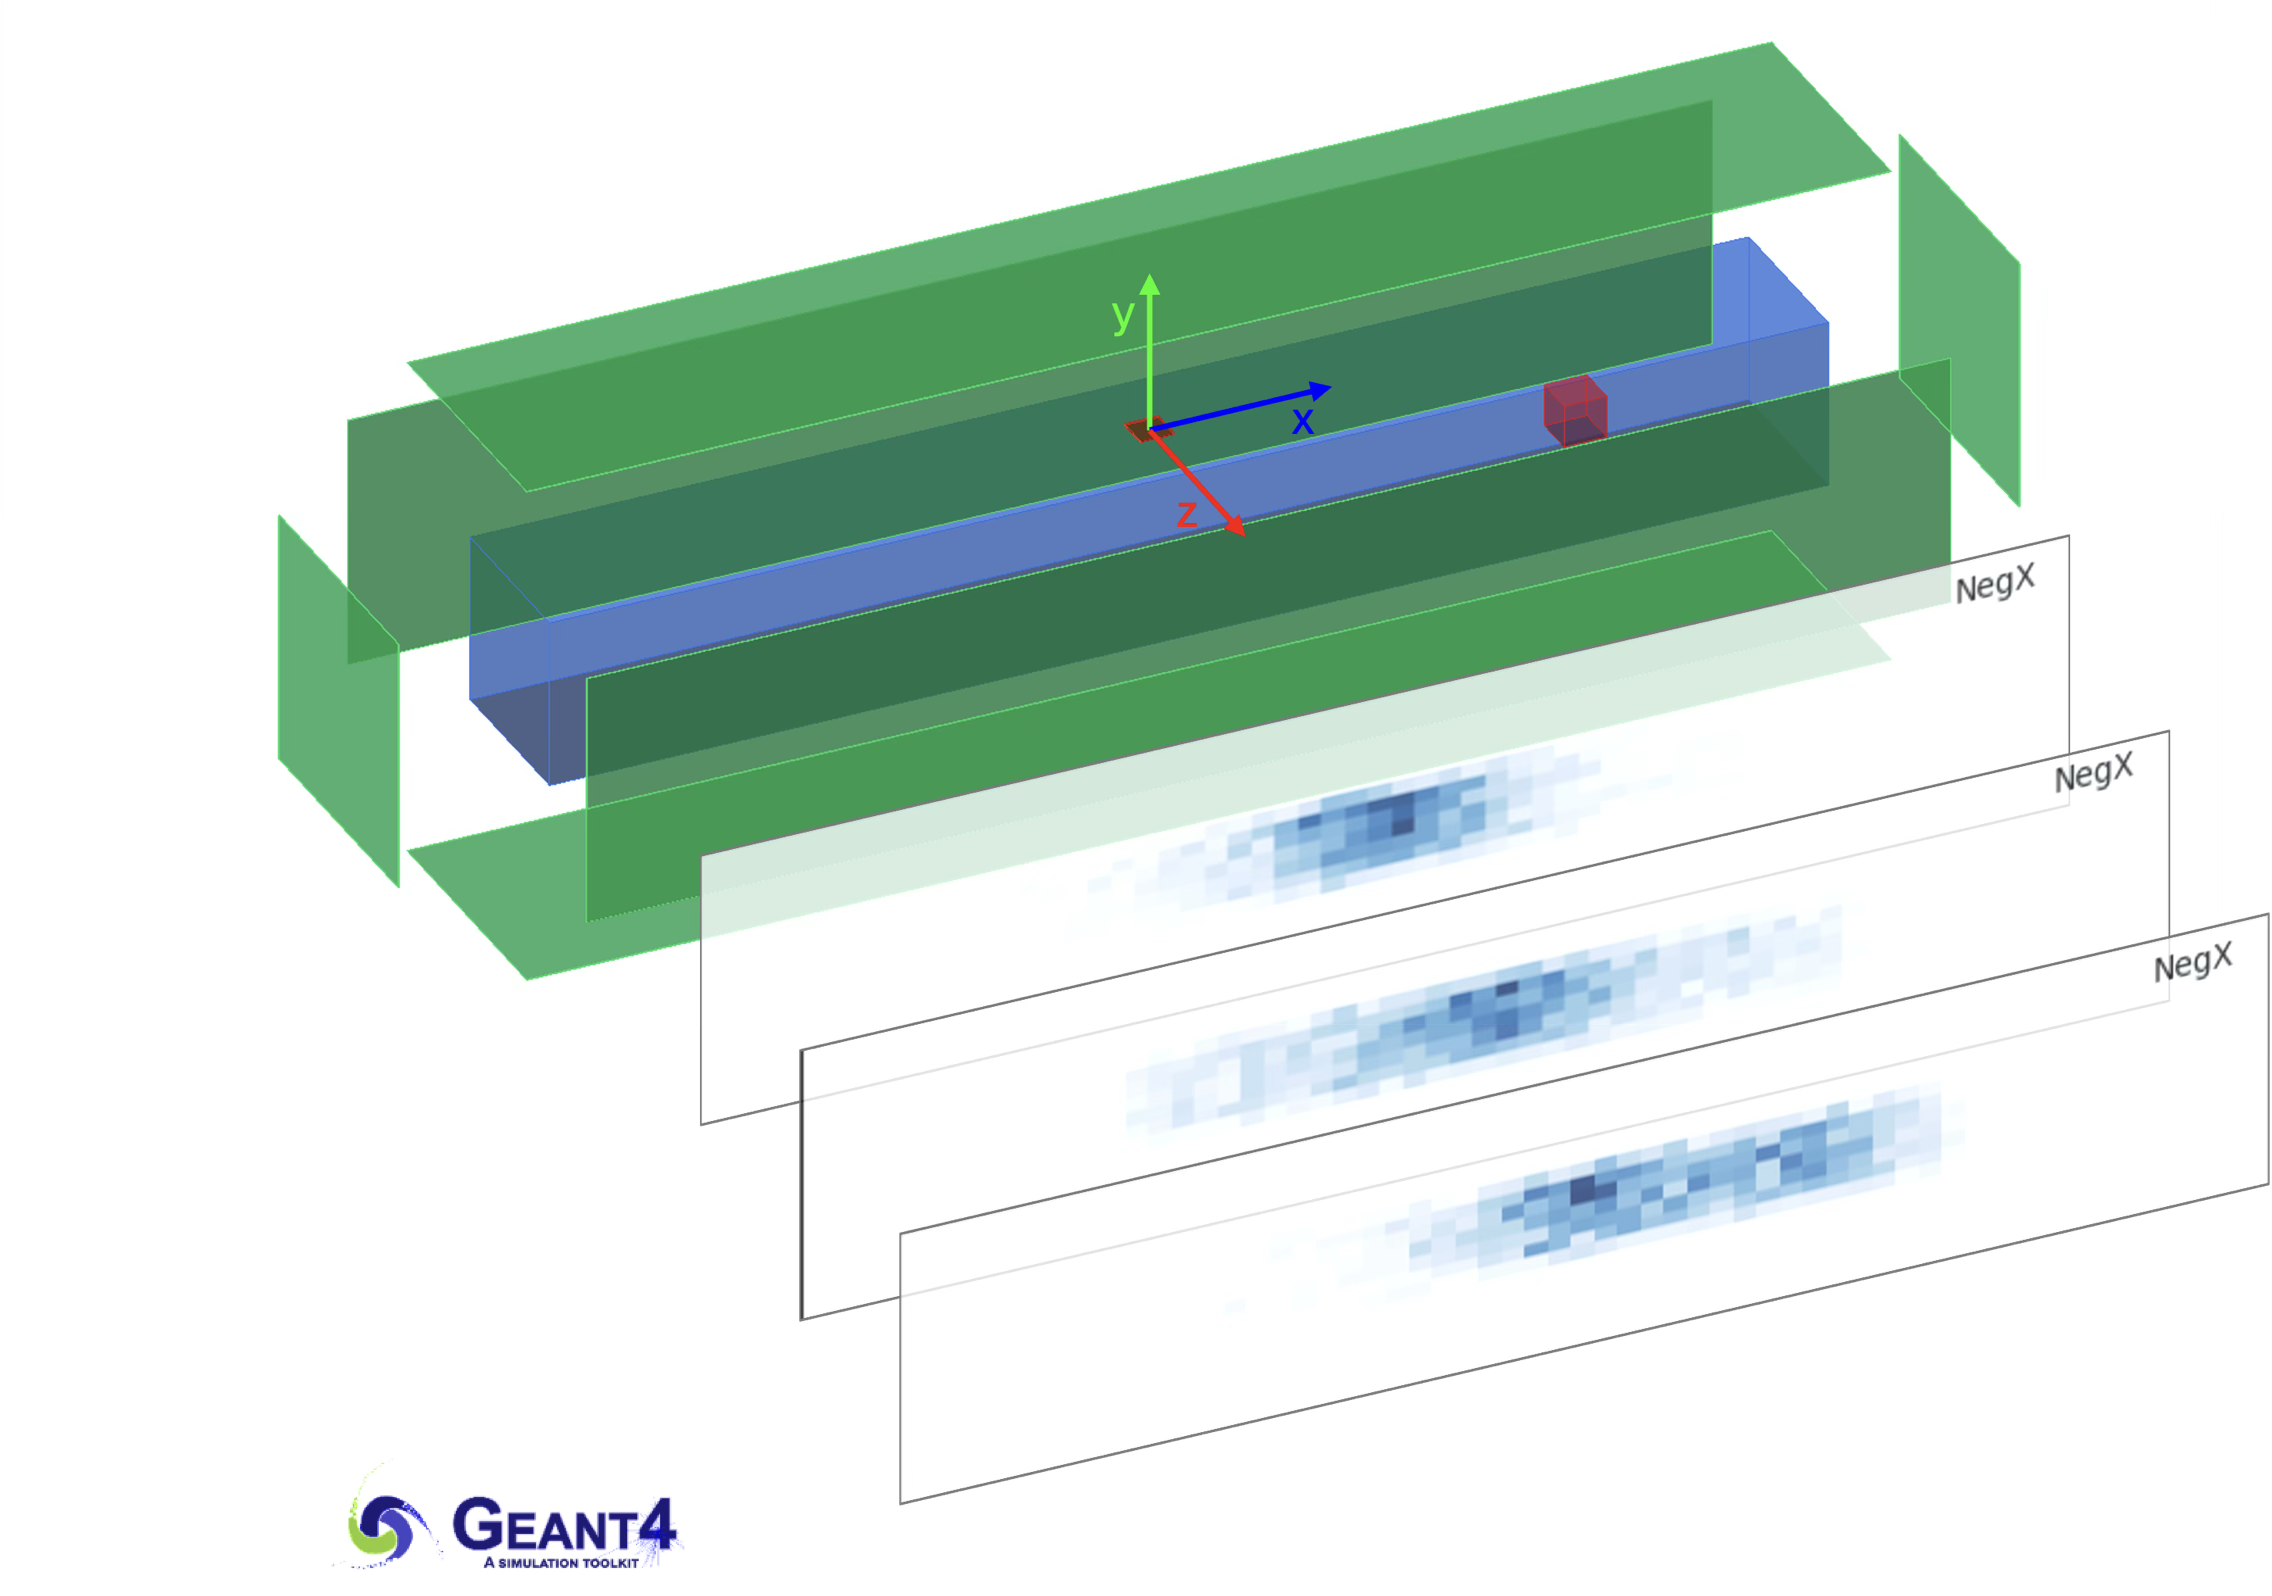
\includegraphics[width=0.88\linewidth]{aocmp_poster_geometry.png}
    \caption{\textit{Simulation geometry showing the water phantom (blue),
    surrounding detector panels (green), a displaced source (red), and
    example detector projections.}}
    \label{fig:abs_geometry}
\end{figure}

\subsection*{Baseline subtraction}

The total detector-entry rate changed only weakly between retained and
redistributed source states.  The total detector-entry rate changed by only
about 3.8\% between the retained
baseline and the 90\% broad-diffusion case.  In contrast,
baseline-subtracted profiles show a clear spatial signature.  The retained
source defines the reference profile \(\bar{h}^{B}_{p}(z)\) for each detector
panel \(p\).  Candidate source states are represented by residuals
\[
  \Delta h_p(z) = h_p(z) - \bar{h}^{B}_{p}(z),
\]
with the repeated baseline simulations defining the bin-wise noise scale.
Positive residuals mark detector regions where the candidate produces more
gamma entries than the retained-source case; negative residuals mark depleted
regions.  Broad diffusion widens the residual pattern and changes the balance
between the glue-facing and opposite detector panels, while localised
displacement produces a shifted excess near the displaced source region.
\begin{figure}[!bp]
    \centering
    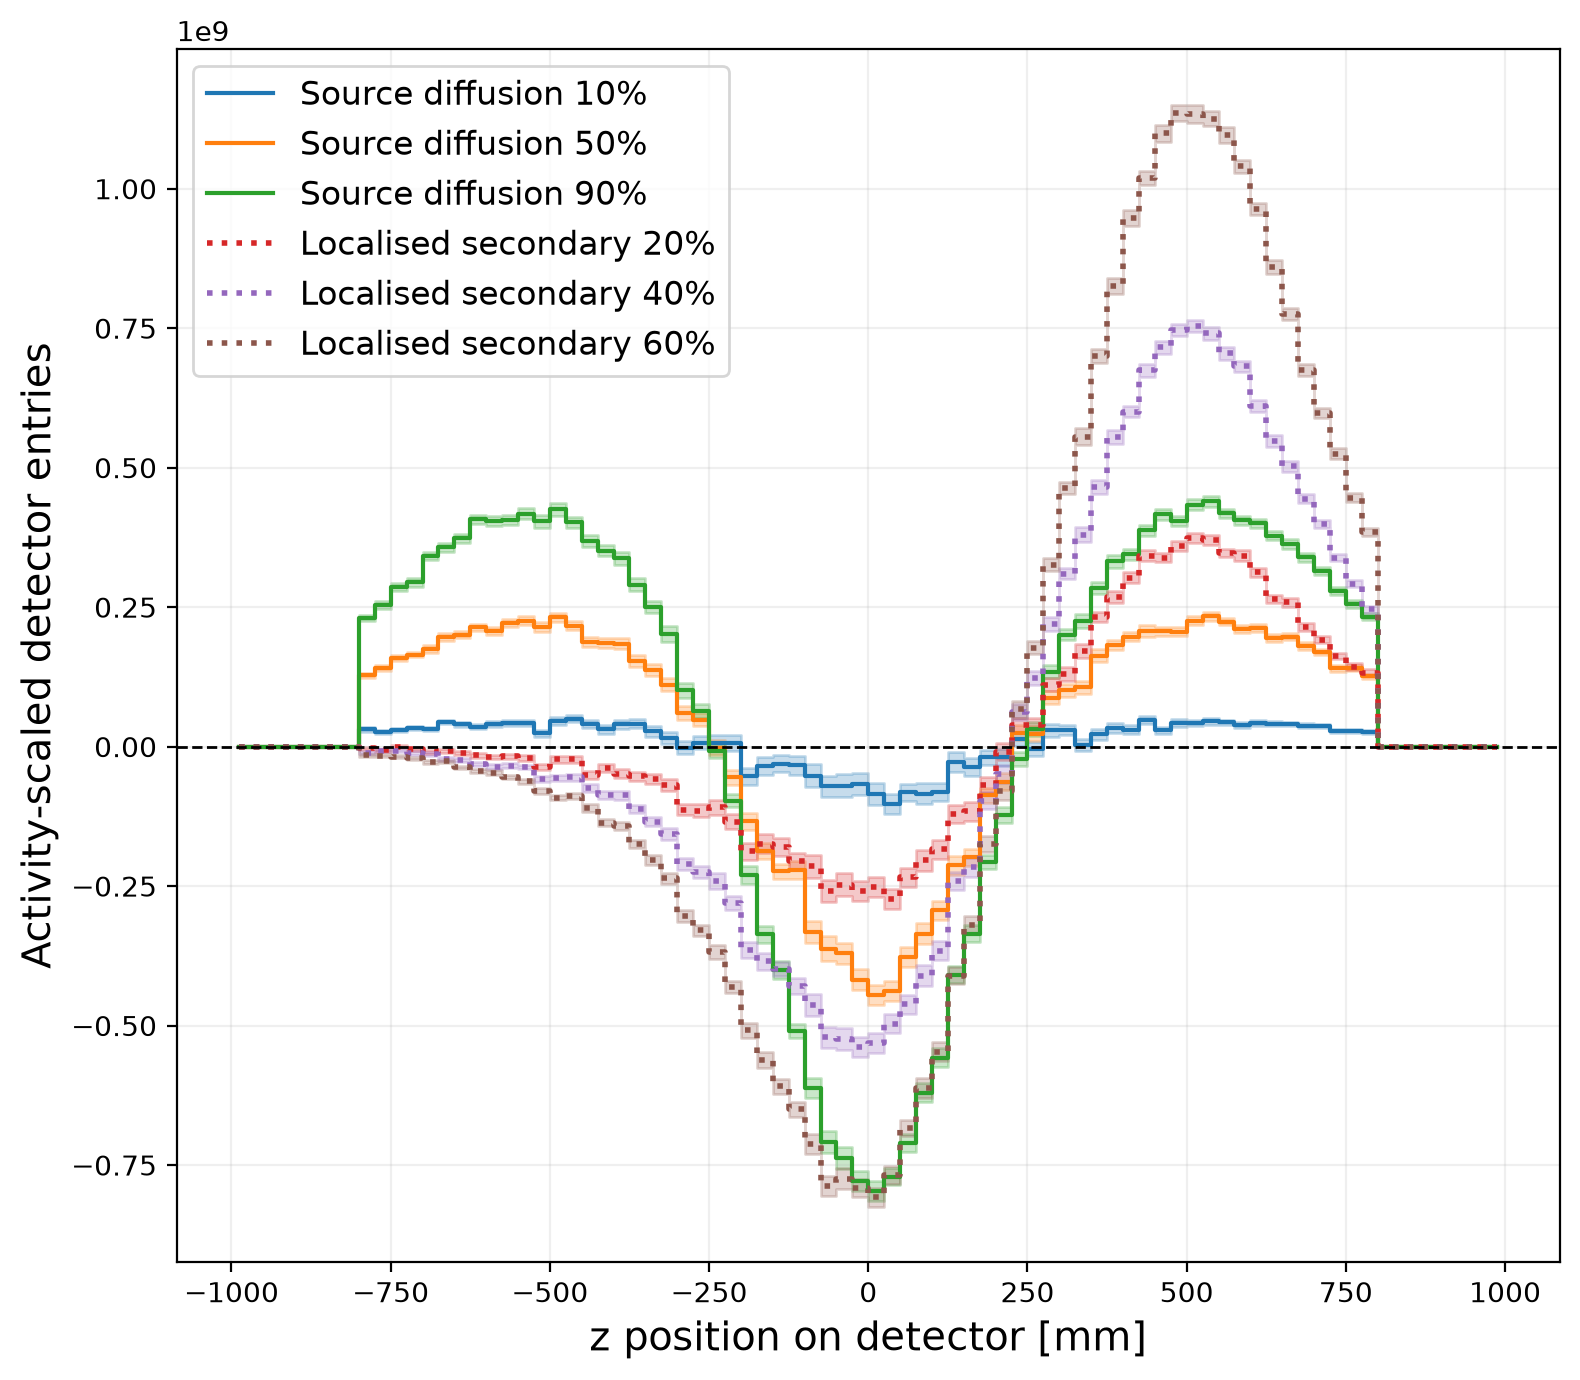
\includegraphics[width=\linewidth]{../figures/signal_analysis_50reps/poster_01_baseline_subtracted_profiles_xsum_all_cases.png}
    \caption{\textit{Activity-normalised, baseline-subtracted \(+x\) and
    \(-x\) detector profiles for broad diffusion and localised displacement.
    Shaded bands show variation across repetitions.}}
    \label{fig:abs_x_profile}
\end{figure}
This indicates that source movement is better detected from
baseline-subtracted spatial hit patterns than from the total hit rate alone
(Fig.~\ref{fig:abs_x_profile}).

\subsection*{Residual-based source metrics}

The residual analysis was organised into three source-monitoring metrics.
First, diffusion was inferred from profile-shape features and panel-balance
changes.  The \(+y\) panel response decreases as activity moves away from the
glue layer, while the profile width and the side-panel share increase.
Second, activity-retention observables used the central \(+y\) region of
interest as an applicator-facing signal.  This estimates activity still
consistent with the retained-source geometry, but is interpreted only after a
secondary-source test because compact displaced activity can also suppress
the central signal (Fig.~\ref{fig:abs_central_roi}).  Third, compact
secondary sources were searched for using positive residuals in a
displaced-region ROI and panel-asymmetry changes that are small for broad
diffusion but large for off-applicator localisation.

\begin{figure}[!tbp]
    \centering
    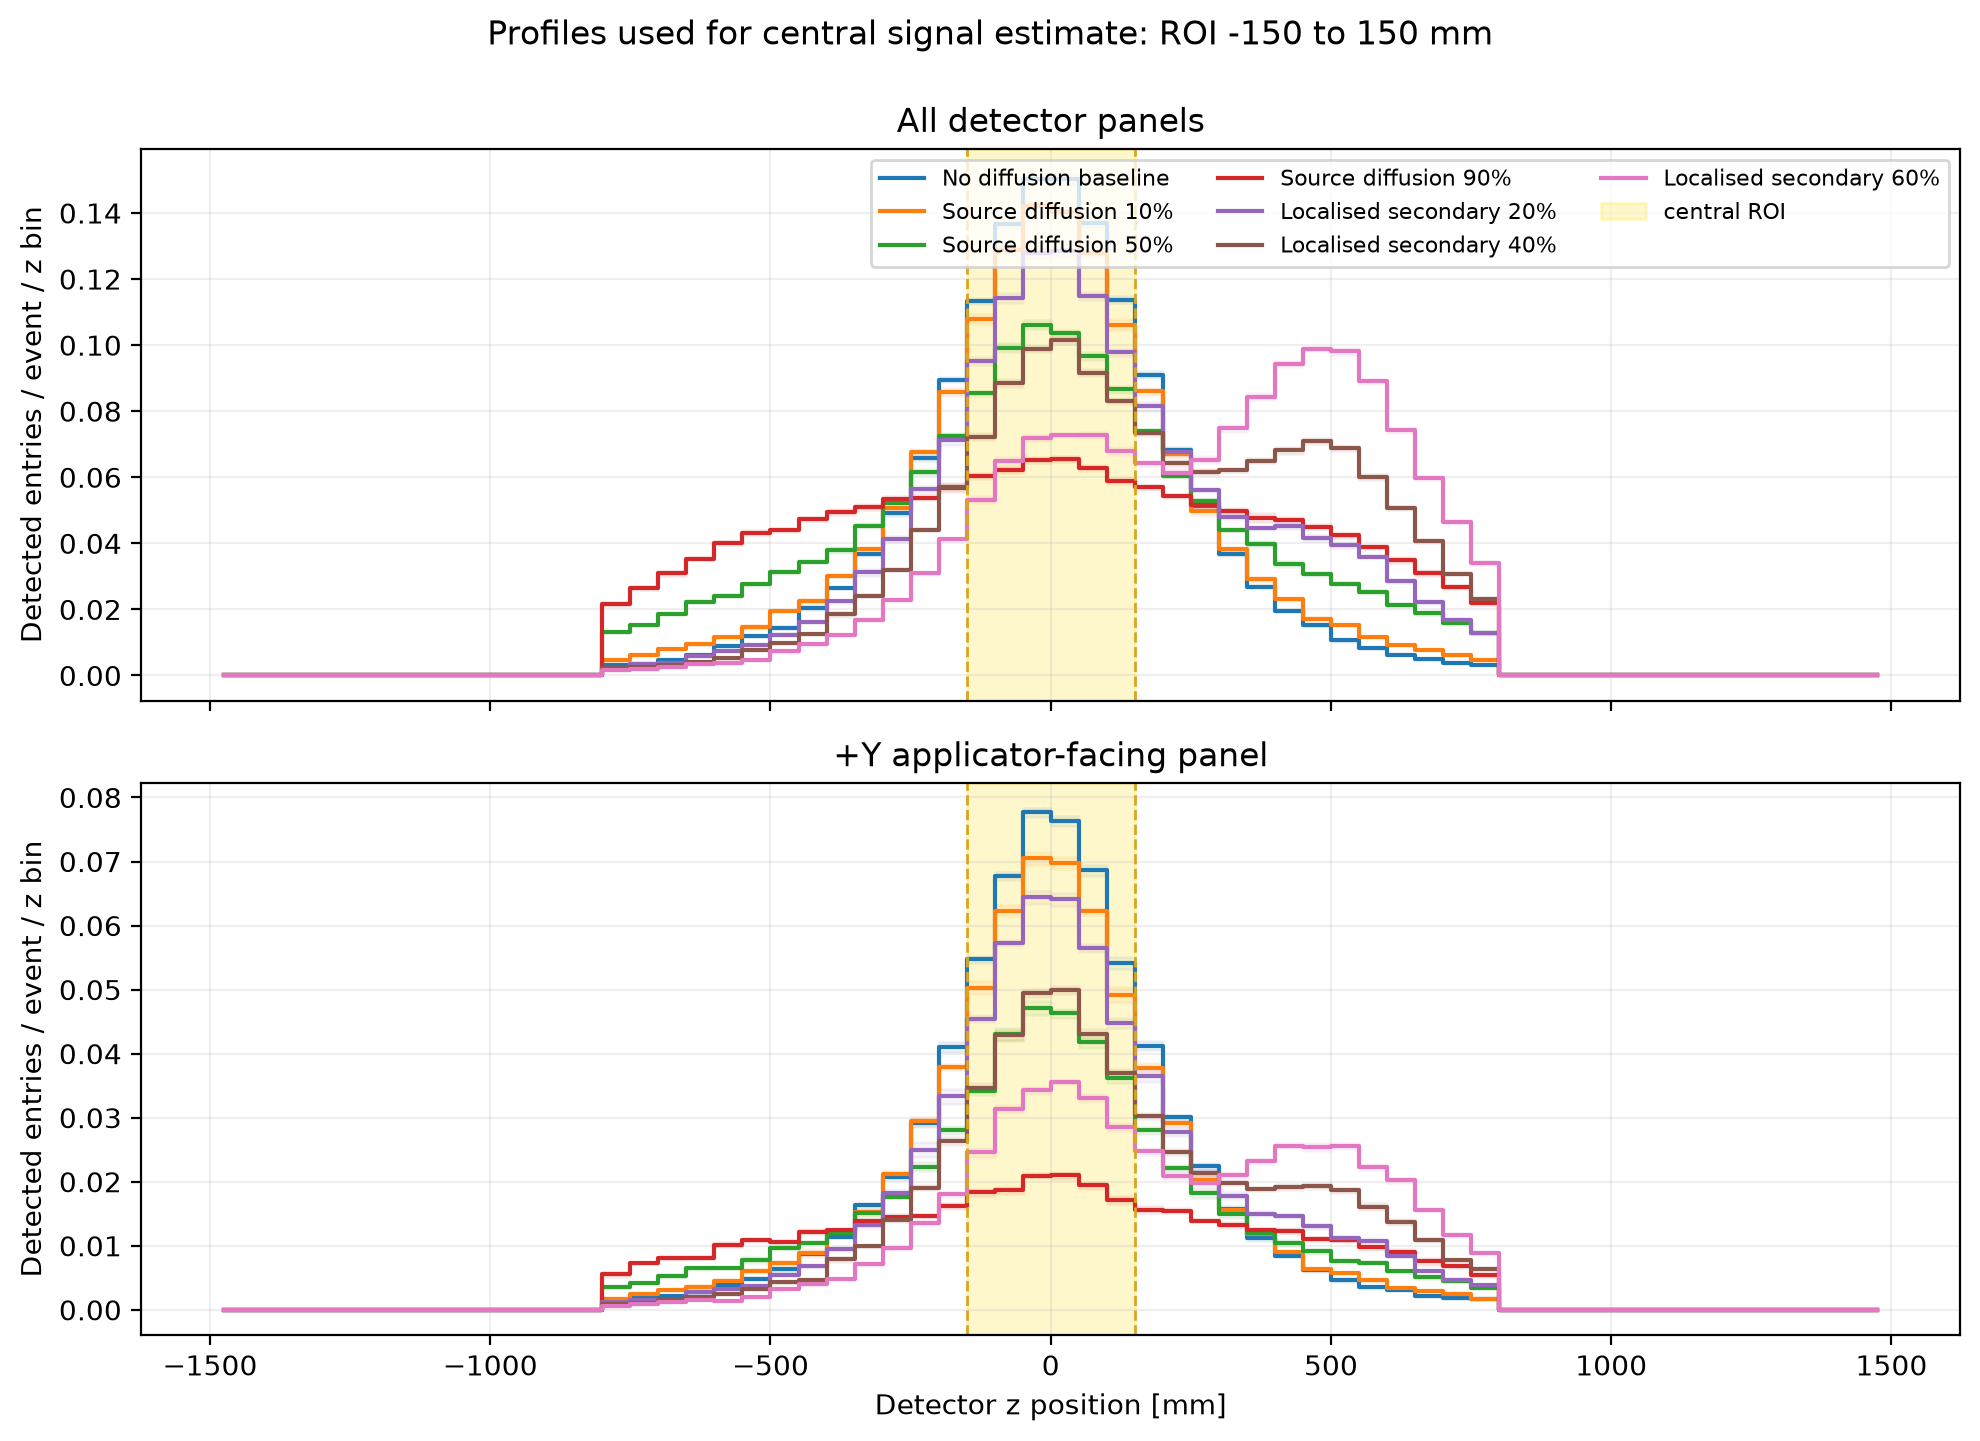
\includegraphics[width=\linewidth]{material_signal_central_roi_profiles.png}
    \caption{\textit{Central-ROI signal used to separate retained applicator
    response from activity redistributed outside the applicator region.}}
    \label{fig:abs_central_roi}
\end{figure}

\begin{figure*}[!tbp]
    \centering
    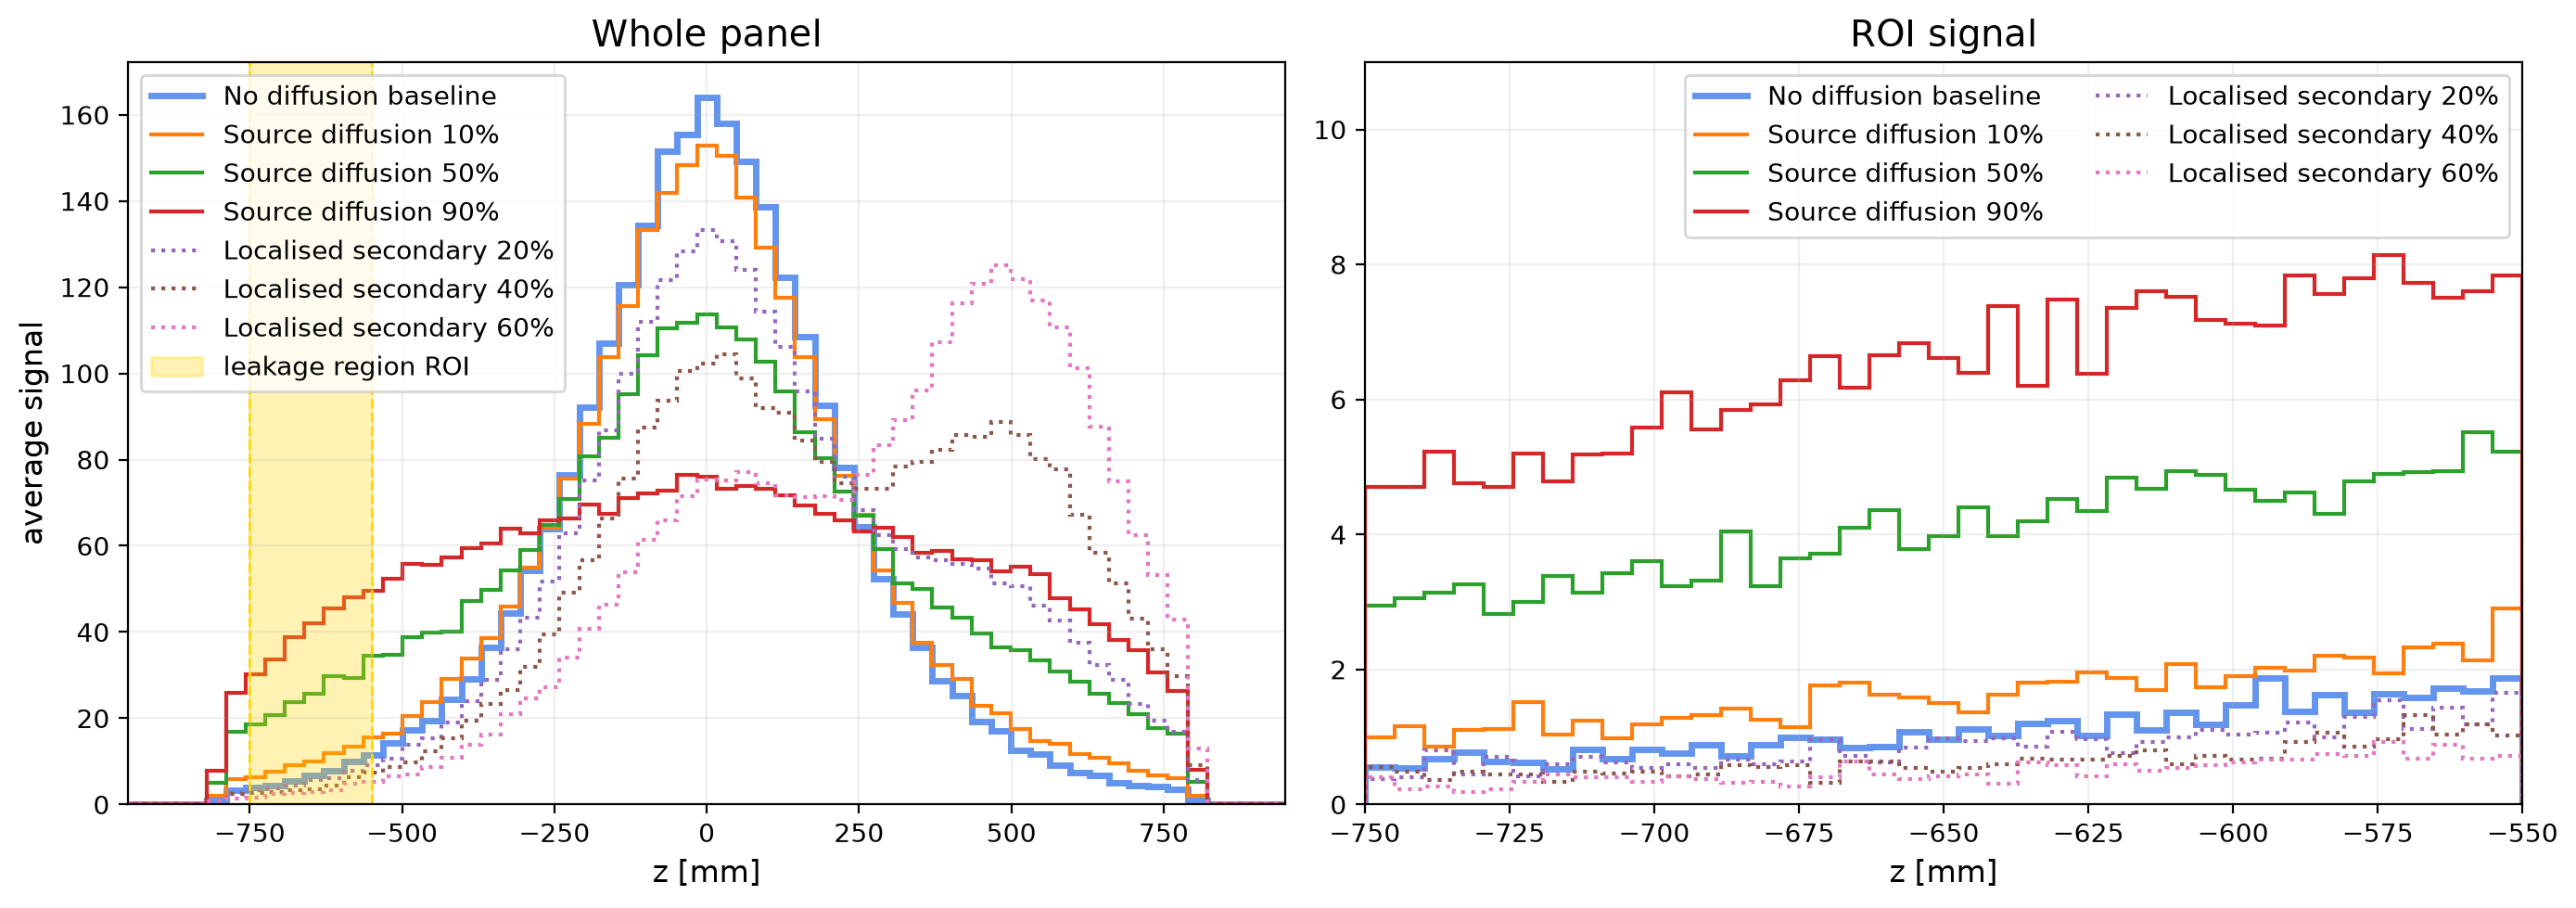
\includegraphics[width=0.94\textwidth]{../figures/signal_analysis_50reps/poster_03c_leakage_roi_side_by_side.png}
    \caption{\textit{Whole \(x\)-panel profiles
    (left) and the displaced-region ROI signal (right). The ROI highlights
    the broad-diffusion excess outside the retained-source region.}}
    \label{fig:abs_leakage_roi}
\end{figure*}

For the present geometry, the displaced-source search ROI is centred on the
positive-\(z\) region containing the simulated compact water source.  The
secondary-source score integrates the positive residual in this ROI and
compares it with the retained-source baseline variation.  If this test is
positive, the location is estimated from the positive-residual centroid on
the detector views that best project the source onto the longitudinal axis.
This cascade is important: diffusion fraction is reported for broad
redistribution candidates, while localised cases are first reported as
compact secondary-source detections with an estimated position.  The leakage
comparison is shown in Fig.~\ref{fig:abs_leakage_roi}.

\subsection*{Signal inference}

Using profile-shape features from repeated simulations, the broad
diffusion fraction was recovered with \(R^2=0.9987\) and a mean absolute
error of about one percentage point. 
A separate secondary-source
metric identified the localised displaced source in all 20\%, 40\%, and
60\% localised-displacement cases.  The reconstructed displaced-source
positions were approximately \(z=\SI{516}{mm}\), \(\SI{528}{mm}\), and
\(\SI{530}{mm}\) for 20\%, 40\%, and 60\% localised activity, respectively,
compared with the simulated \(z=\SI{500}{mm}\) source region.  Across these
localised fractions, mean position errors were \(16\)--\(\SI{30}{mm}\)
(Figs.~\ref{fig:abs_diffusion_prediction}
and~\ref{fig:abs_source_residuals}).

\begin{figure}[!tbp]
    \centering
    \includegraphics[width=\linewidth]{../figures/signal_analysis_50reps/poster_02_diffusion_fraction_cv_prediction.png}
    \caption{\textit{Diffusion fraction inferred from 50 independent
    repetitions; points show individual repetitions and large
    markers show the mean and standard deviation.}}
    \label{fig:abs_diffusion_prediction}
\end{figure}

\begin{figure*}[!tbp]
    \centering
    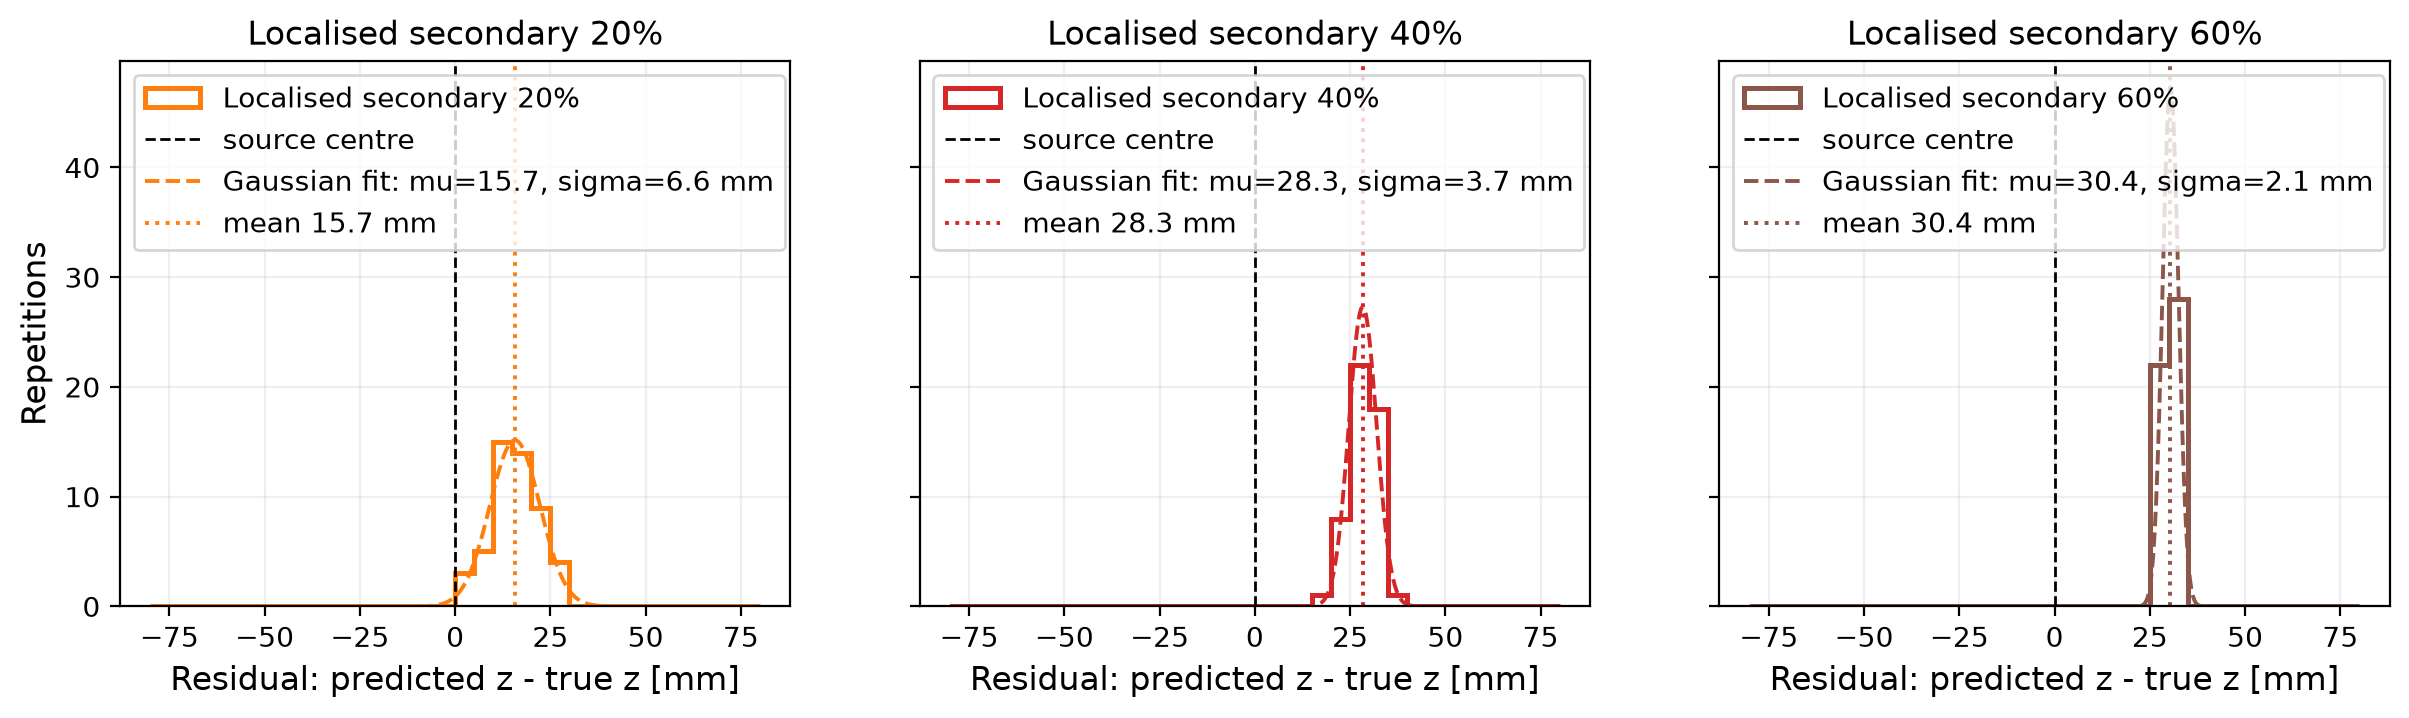
\includegraphics[width=0.94\textwidth]{../figures/signal_analysis_50reps/poster_04b_localised_source_position_residuals.png}
    \caption{\textit{Localisation residuals across 50 repetitions for
    each displaced-source fraction. The dashed black line marks the true
    source centre; coloured lines indicate the mean and Gaussian fit.}}
    \label{fig:abs_source_residuals}
\end{figure*}

\subsection*{Time dependence}
Cumulative time-window profiles show that the baseline-subtracted signal is
already visible on hour-scale windows and becomes stronger over longer
observation windows.  Across the 50 repetitions, detectability
required candidate-baseline separation greater than \(3\sigma\) of the
run-to-run baseline variation.  The 50--90\% broad-diffusion and 20--60\%
localised-displacement cases crossed threshold in about 1--2 hours, while
the weaker 10\% broad-diffusion case required about 6 hours.  A
representative time-window profile and a separate ROI significance
trajectory are shown in Fig.~\ref{fig:abs_time_windows}.  A
\(t<10^6~\mathrm{s}\) analysis cut suppresses a late decay-chain tail while
retaining the early signal relevant to the simulated source-localisation
window.

\begin{table}[!tbp]
\centering
\scriptsize
\caption{\textit{Summary of first \(3\sigma\) detection times from the
time-window analysis of 50 independent repetitions.}}
\label{tab:time_detection}
\begin{tabular}{lc}
\toprule
Case group & First \(3\sigma\) detection \\
\midrule
10\% broad diffusion & about 6 h \\
50--90\% broad diffusion & about 1--2 h \\
20--60\% localised displacement & about 1--2 h \\
\bottomrule
\end{tabular}
\end{table}

\begin{figure*}[!tbp]
    \centering
    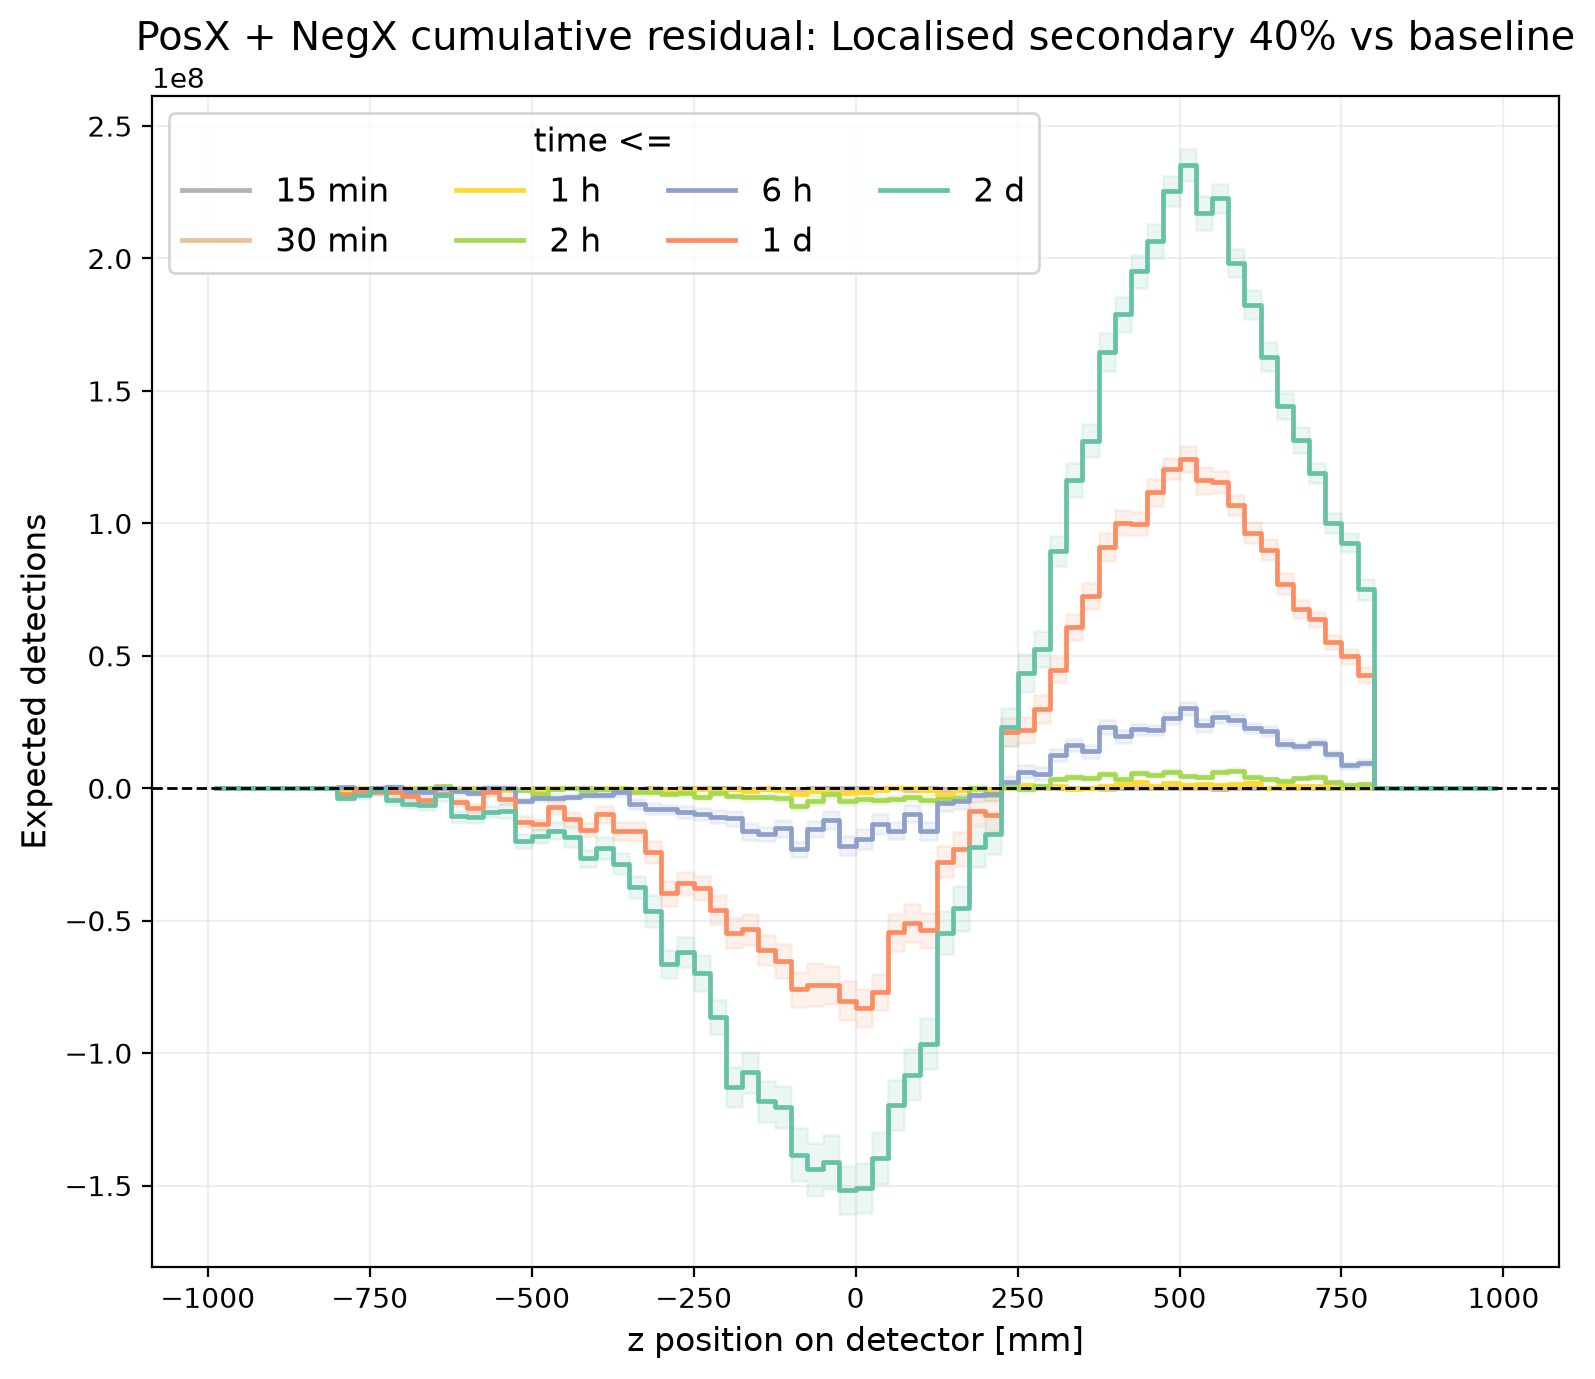
\includegraphics[width=0.46\textwidth]{../figures/signal_analysis_50reps/poster_05_time_window_residual_profiles_loc40.png}\hfill
    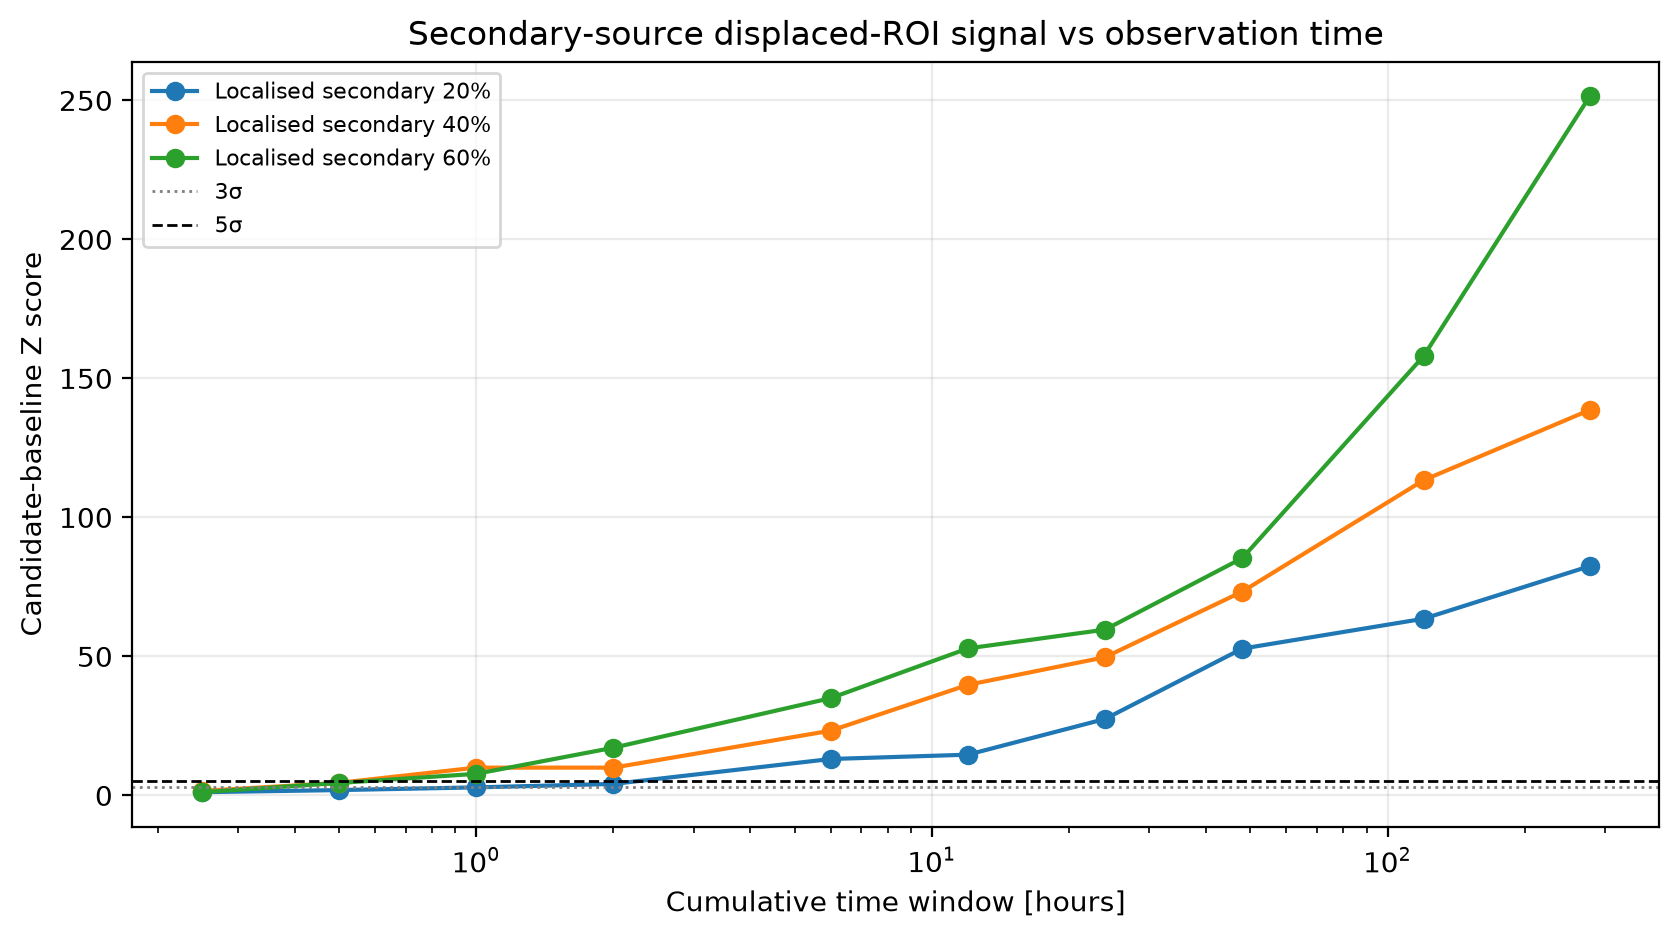
\includegraphics[width=0.46\textwidth]{secondary_displaced_roi_zscore_vs_time.png}
    \caption{\textit{Time-dependent residual analysis. Left: the
    cumulative \(+x\) and \(-x\) profile for 40\% localised displacement,
    showing a growing excess near \(z=\SI{500}{mm}\). Right: significance of
    the distinct displaced-source ROI signal with observation time.}}
    \label{fig:abs_time_windows}
\end{figure*}
\subsection*{Outlook}

These results indicate that decay-chain gamma detection can provide
source-location information that is not captured by total count rate alone.
Further work will include detector response, backgrounds, and patient-scale
geometries so that the activity-normalised profiles can be interpreted as
experimentally measurable count rates.

\subsection*{References}
{\small
\scriptsize
\begin{thebibliography}{1}
\bibitem{AlphaGlue2025}
L. Abu Sabah \textit{et al.}, ``AlphaGlue: A Novel Conceptual Delivery
Method for \(\alpha\) Therapy,'' \textit{BioMedInformatics} 5, 58, 2025.
\bibitem{laura}
L. Ballisat \textit{et al.}, ``Geant4 simulation of the enhanced in-vivo
\(^{220}\)Rn spread in DaRT,'' \textit{Phys. Med.} 135, 105005, 2025.
\bibitem{heger}
G. Heger \textit{et al.}, ``First measurements of radon-220 diffusion in
mice tumors,'' \textit{Med. Phys.} 51, 5045--5058, 2024.
\bibitem{Geant4}
S. Agostinelli \textit{et al.}, ``Geant4---a simulation toolkit,''
\textit{Nucl. Instrum. Methods Phys. Res. A} 506, 250--303, 2003.
\bibitem{dart}
L. Arazi \textit{et al.}, ``The treatment of solid tumors by alpha emitters
released from \(^{224}\)Ra-loaded sources,'' \textit{Phys. Med. Biol.} 55,
1203, 2010.
\bibitem{Geant4DNA}
S. Incerti \textit{et al.}, ``The Geant4-DNA project,''
\textit{Int. J. Model. Simul. Sci. Comput.} 1, 157--178, 2010.
\end{thebibliography}
}

\end{document}
